\section{Project Plan}
\label{sec:projectplan}
To provide a schedule and to check whether the project is still proceeding at a good pace, a project plan has been developed after performing the requirements analysis and discussing various aspects of the project with the client (the main author of the paper summarised in \autoref{sub:statistical_model_selection}). This project plan can be found as a Gantt-Chart in \autoref{fig:projectplan}. In general, light blue colour is used for tasks related to the actual thesis (writing, reports, research). Blue coloured tasks represent requirement, analysis and development tasks. Light green tasks are related to project reports whereas dark-green tasks stand for feedback cycles. Green milestones (diamonds) represent internal release candidates of the development iterations. Red milestones represent external milestones and due dates. The overall development process is structured in four Release Cycles RC1 - RC4. 

This schedule was updated according to the actual progress of the project, \autoref{fig:projectplan} shows the most recent updated version. Updates on it where necessary because of various reasons:

First of all, the different project phases have changed: The writing of the final thesis has been postponed and the focus on the development has been increased during the first months. In addition as a learning from RC 1, the duration of the different release candidates have been reduced to iterate faster. A buffer of approximately 4 weeks has been integrated into the planning to be able to react flexible on problems that might occur during the development. 

Other than that the feedback times have been decoupled from the remaining development process, as we decided to have short demo sessions immediately after each release candidate, therefore the feedback process could be reduced to a minimum.

\newgeometry{bottom=1.5cm}
\begin{sidewaysfigure}[h]
	\centering
	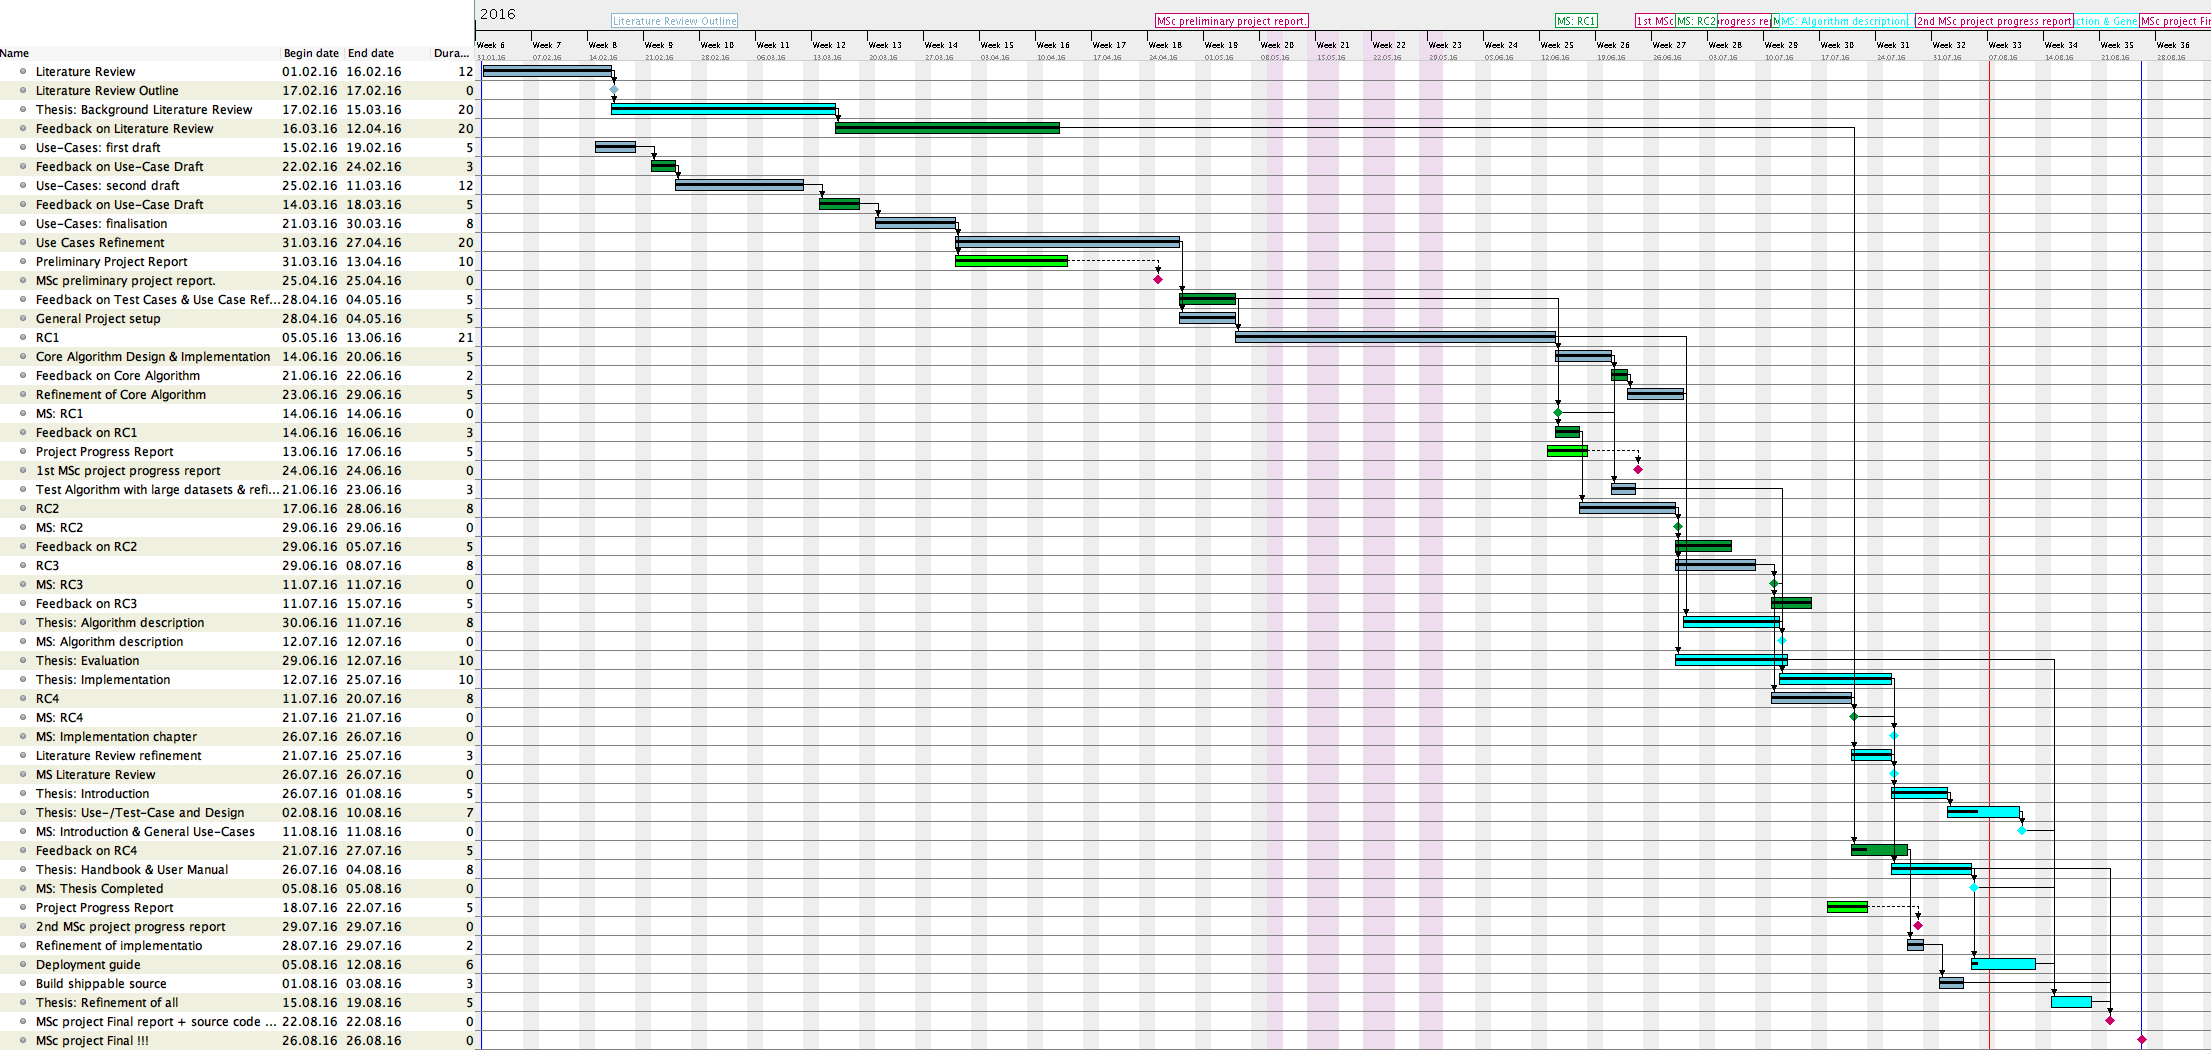
\includegraphics[width=\textwidth]{appendix/Projectplan}
	\caption{Project plan for the whole development and research.}
	\label{fig:projectplan}
\end{sidewaysfigure}
\restoregeometry